\documentclass[12pt,a4paper]{article}
\usepackage[polish]{babel}
\usepackage[a4paper,top=2cm,bottom=1.5cm,left=2cm,right=2cm,marginparwidth=1.75cm]{geometry}
\usepackage[T1]{fontenc}
\usepackage[MeX]{polski}
\usepackage{amsmath}
\usepackage{graphicx}
\usepackage{caption}
\usepackage[colorlinks=true, allcolors=blue]{hyperref}
\usepackage[utf8]{inputenc}
\usepackage{lmodern}
\usepackage{color}
\usepackage{colortbl}
\usepackage{multirow}
\usepackage{listings}
\usepackage{hyperref}

\title{Sprawozdanie Projektowe \\ Program ''Sklep''}
\author{Dawid Duma 66722}

\begin{document}
\makeatletter
    \begin{titlepage}
        \begin{center}
            
\includegraphics[width=0.7\linewidth]{figures/logoWSIiZ.png}\\[4ex]
            {\huge \bfseries  \@title }\\[2ex] 
            {\LARGE  \@author}\\[50ex] 
            {\large \today}
        \end{center}
    \end{titlepage}
\makeatother
\thispagestyle{empty}
\newpage

\tableofcontents
\newpage

\section{Wstęp}
Zadanie projektowe polega na zaprojektowaniu programu w języku C\#, który miałby w uproszczony sposób symulować obsługę dowolnego sklepu, tj. sprzedaż oraz przyjecia towarów.

\section{Treść Zadania}
Program „Sklep”. Program ma wspierać obsługę sklepu dowolnego rodzaju. Powinna być możliwość przyjęcia towaru do sklepu oraz jego sprzedaż w sposób hurtowy i detaliczny. Dla sprzedaży hurtowej powinna być możliwość rejestrowania stałych klientów. „Sprzedaż” ma polegać na wybieraniu towarów do koszyka, naliczaniu zbiorczej ceny, zapłatę z pieniędzy posiadanych w portfelu oraz usuwanie „sprzedanych” towarów z magazynu.

\section{Założenia}
W celu realizacji symulacji należy wpierw przygotować listę założeń oraz funkcjonalności programu, tak aby spełniały one wymagania opisane w treści zadania.
	\subsection{Funkcjonalne}
	\begin{itemize}
		\item Sprzedaż klientom indiwidualnym oraz biznesowym (faktury)
		\item Sprzedaż hurtowa 
		\item Możliwośc ustalenia rabatu stałym klientom
		\item Obłsuga przyjęcia towaru na magazyn
		\item Ustalenie stałej marży w zależności od ceny bądź kategorii
	\end{itemize}
	
	\subsection{Niefunkcjonalne}
	\begin{itemize}
		\item Nieograniczony czasowo dostęp do bazy danych
		\item Baza danych dostępna lokalnie (wykorzystanie SQLite)
	\end{itemize}
\newpage

\section{Zarys Aplikacji}
Program wykorzystuje lokalną bazę danych SQLite do zapisywania i odczytywania stanu magazynu oraz historii transakcji. Podczcas pierwszego uruchomienia, bądź gdy baza zostanie usunięta, tworzona jest w folderze domowym użytkownika domyślna, nowa baza o nazwie \verb|SklepBaza.db|. Sama aplikacja pracuje w oknie terminalu, gdzie wykorzystana została biblioteka NCurses, pozwalająca na tworzenie interfejsu użytkownika w owym oknie. Użytkownik nawiguje w oknie za pomocą klawiatury, głównie poperzez predefiniowane wybory widoczne na ekranie. W przypaku pól tekstowy, puste pole oraz kliknięcie klawisza \verb|enter| spowoduje powrot do poprzedniego ekranu.

\section{Uruchamianie}
Program został przewidziany tak, że może zostać uruchomiony na systemach Windows bądź Linux. Zakładając iż środowisko uruchomieniowe .NET jest już zainstalowane i dostępne, to w systemie Linux można uruchomić aplikację poprzez skrypt \verb|start_linux.sh|, za pomocą komendy \verb|dotent run src\\UI\| bądź bezpośrednio w środowisku IDE np. Visual Studio Code. Natomiast aby uruchomić aplikację w systemie Windows należy użyć dołączonego skryptu \verb|start.bat|, tak aby dodatkowe biblioteki, które nie są domyślnie dostępne w tym systemie, mogły zostać załadowane.
\newpage

\section{Prezentacja Funkcjonalności}
\begin{figure}[hp]
\centering

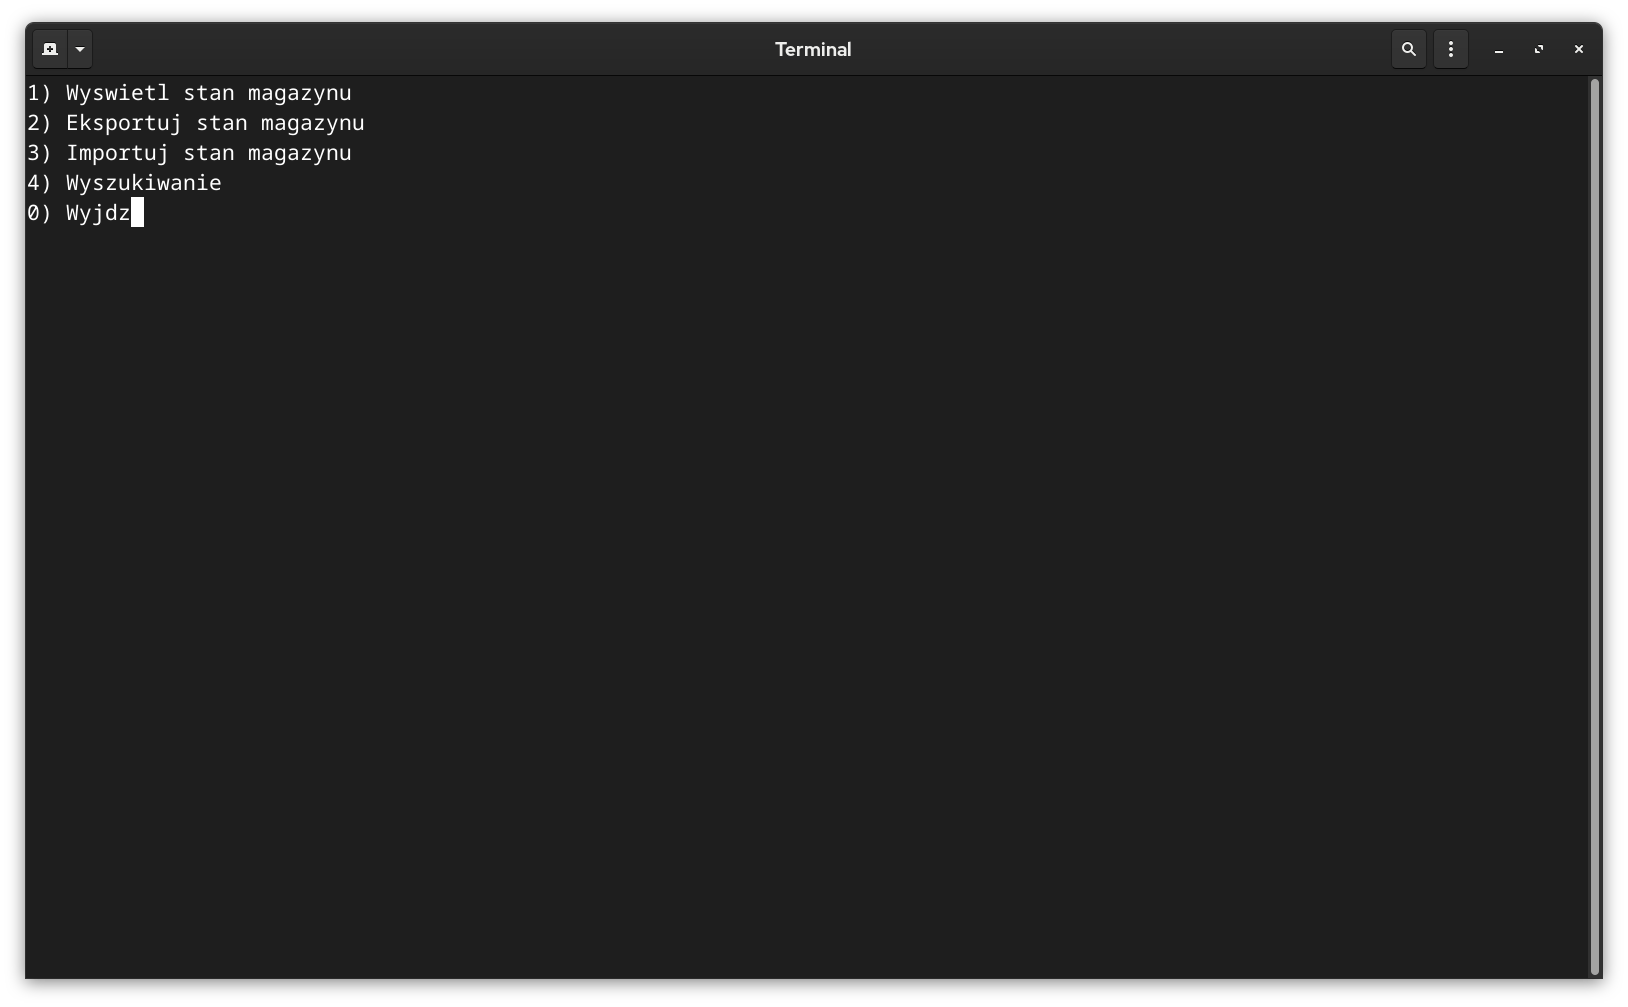
\includegraphics[scale=.30]{figures/ekran_glowny.png}

\caption{Ekran Główny}
\end{figure}

\begin{figure}[hp]
\centering

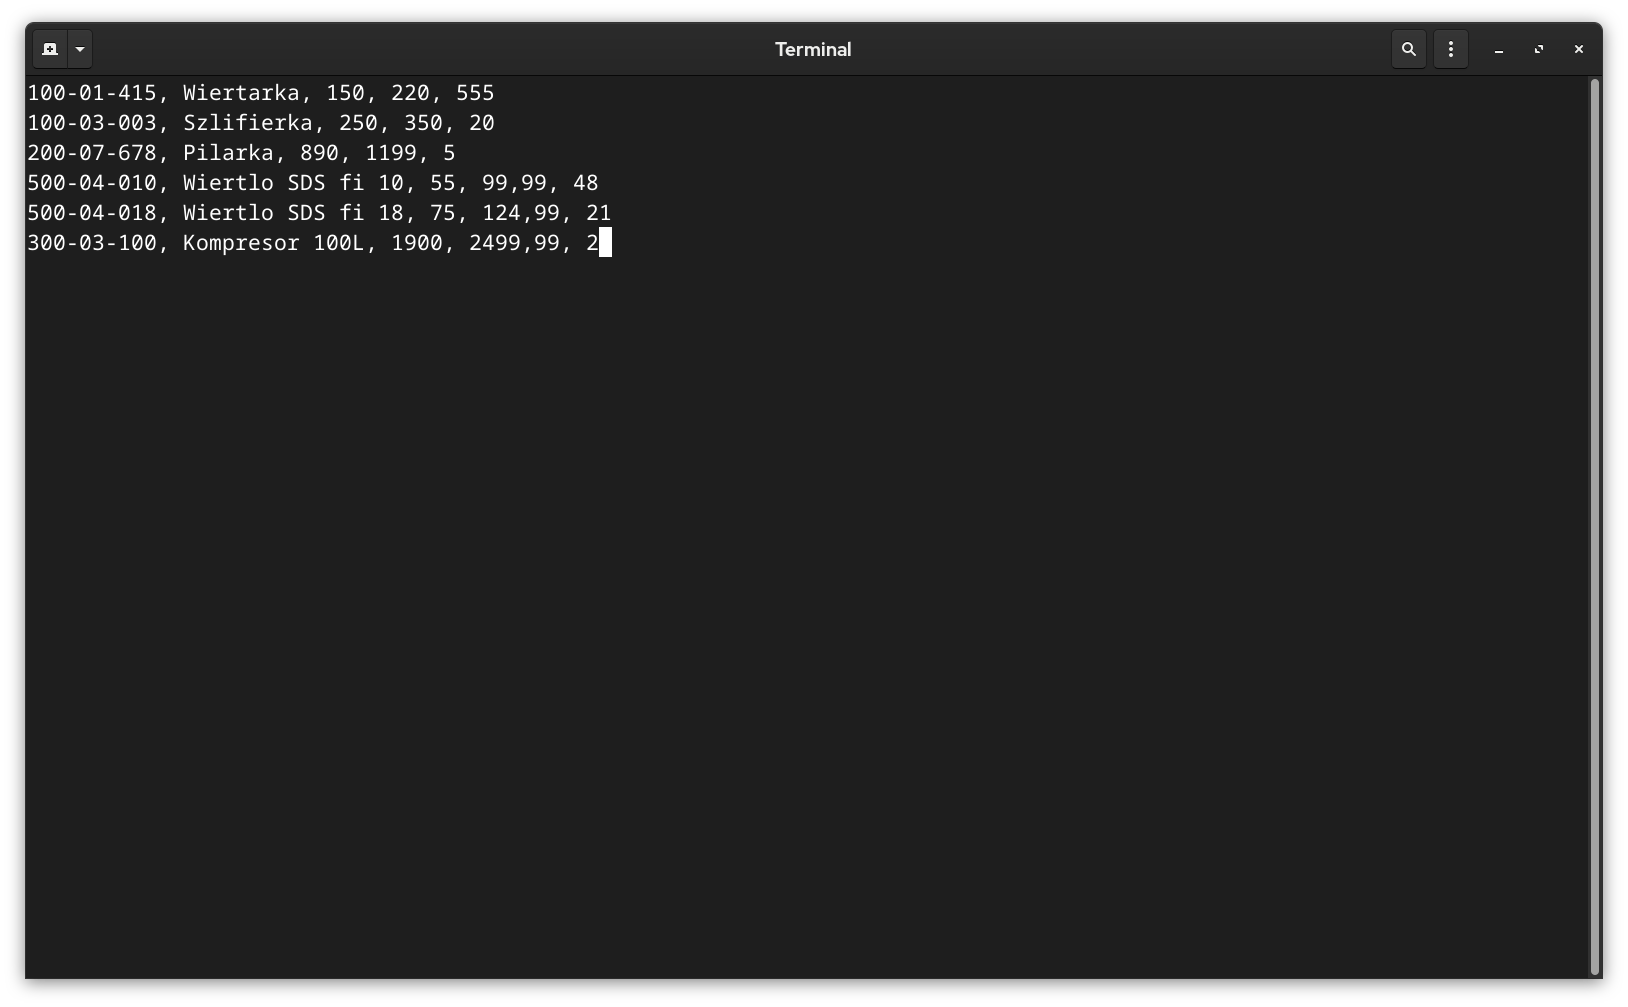
\includegraphics[scale=.30]{figures/ekran_magazynu.png}

\caption{Ekran magazynu}
\end{figure}

\begin{figure}[hp]
\centering

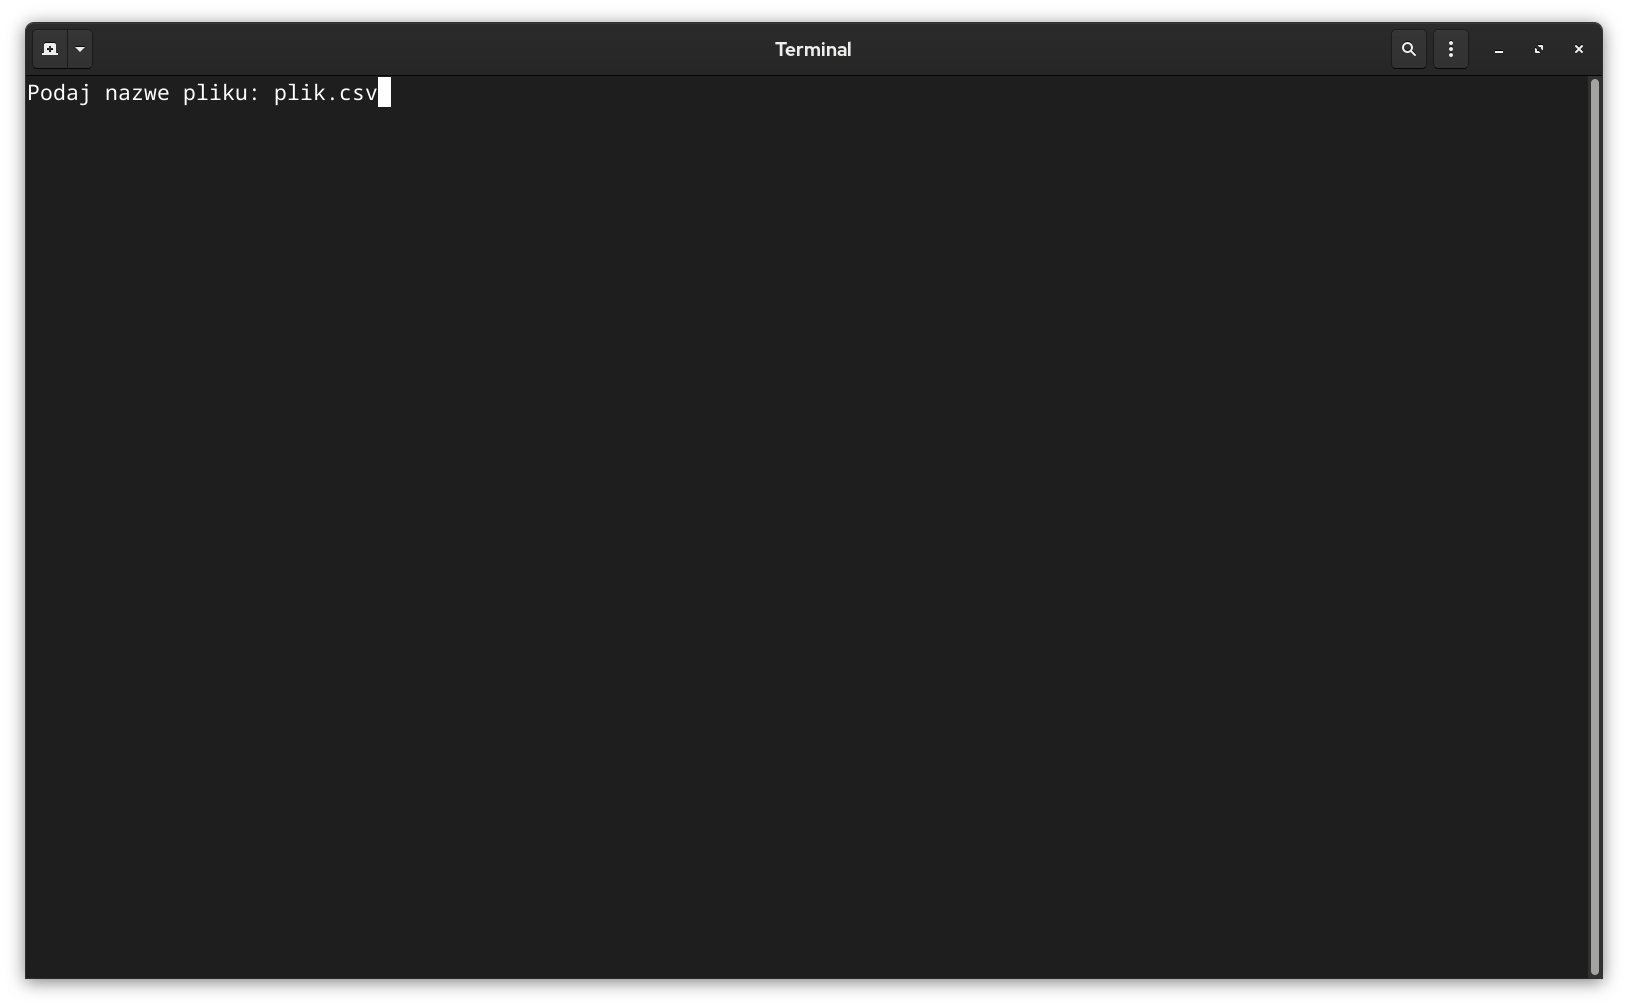
\includegraphics[scale=.30]{figures/ekran_eksportu.png}

\caption{Ekran eksportu}
\end{figure}

\begin{figure}[hp]
\centering

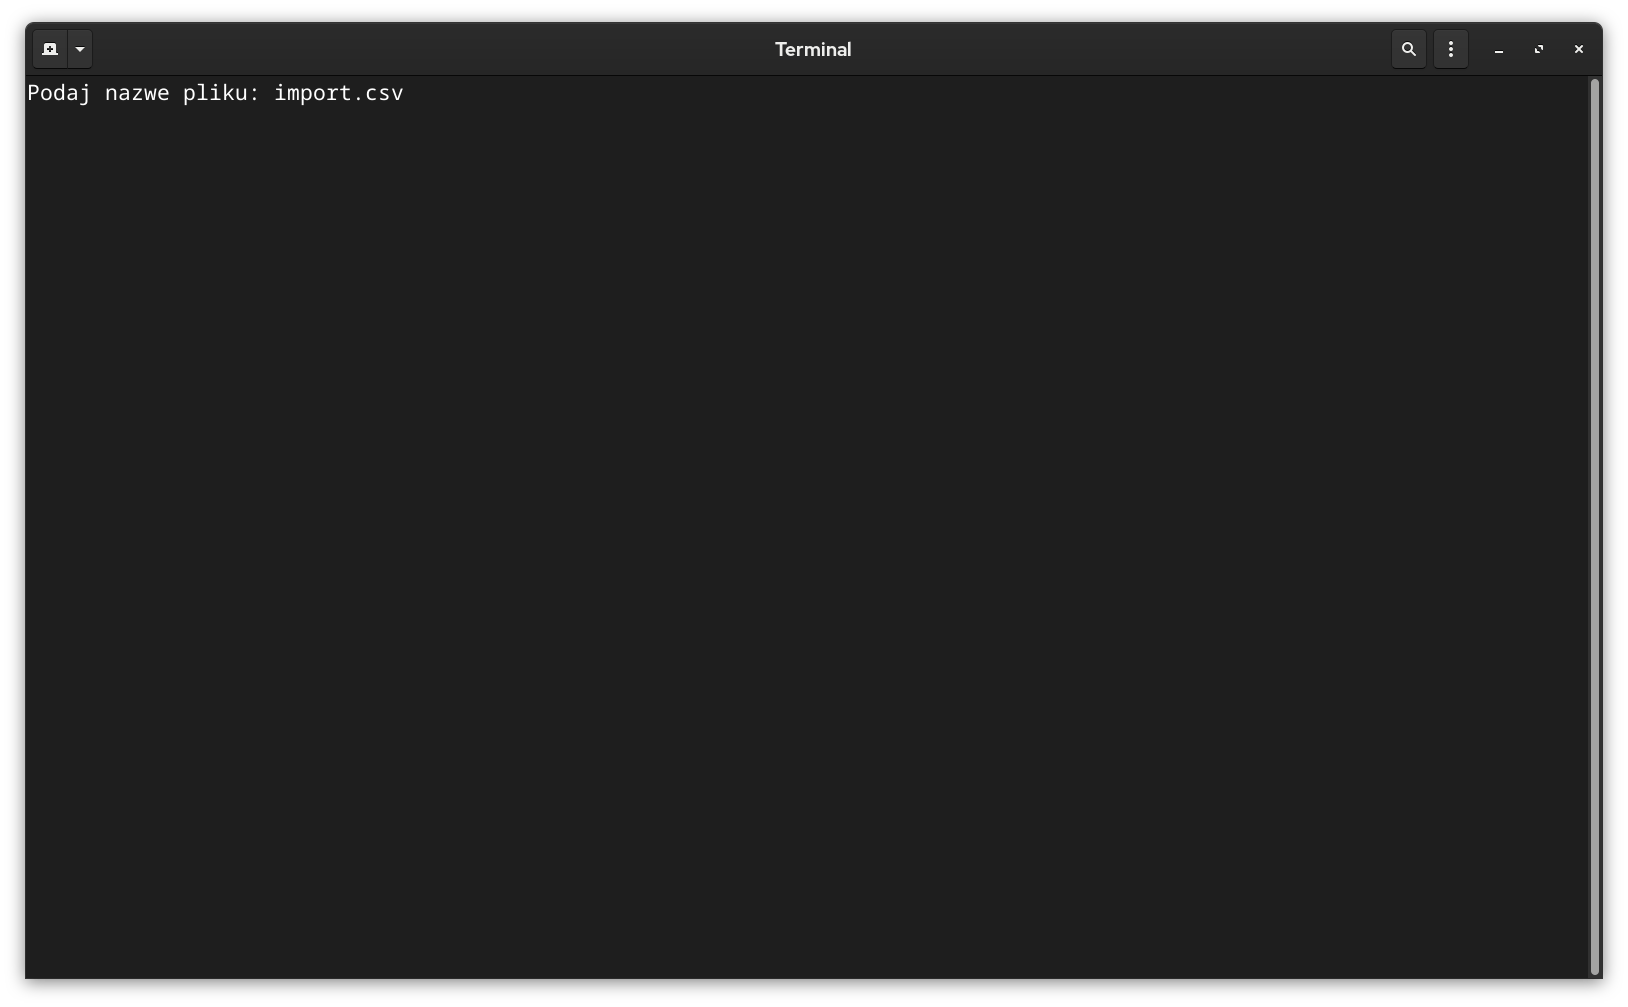
\includegraphics[scale=.30]{figures/ekran_importu.png}

\caption{Ekran importu}
\end{figure}

\begin{figure}[hp]
\centering

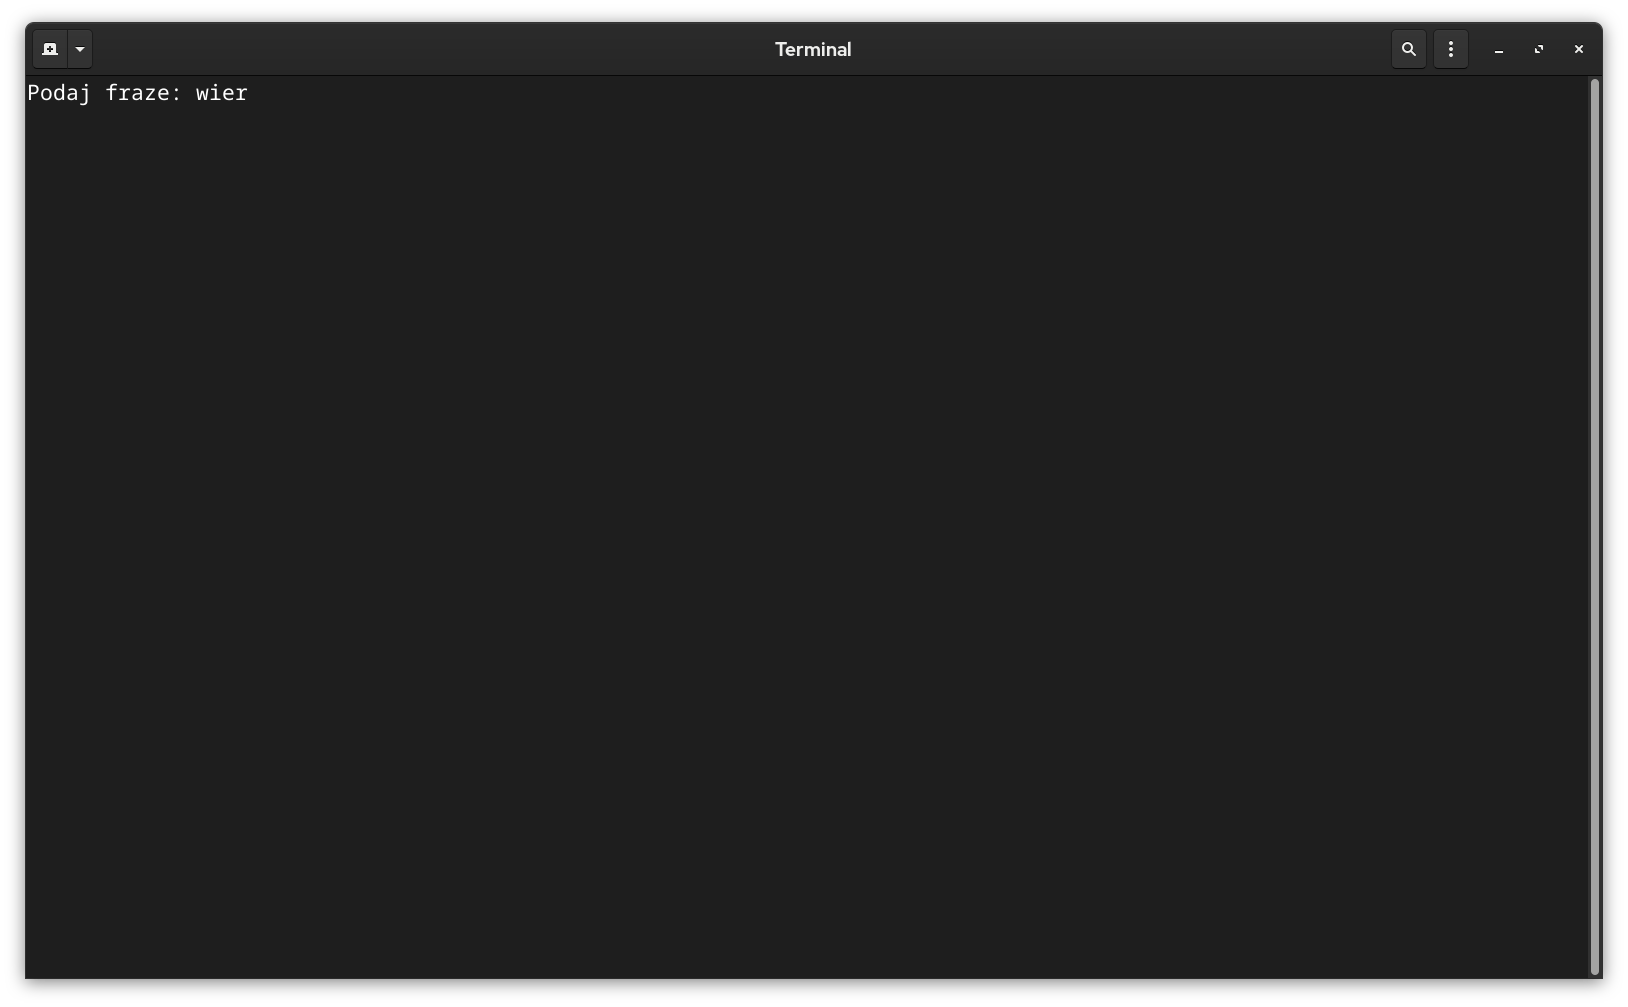
\includegraphics[scale=.30]{figures/ekran_wyszukiwania.png}

\caption{Ekran wyszukiwania}
\end{figure}

\begin{figure}[hp]
\centering

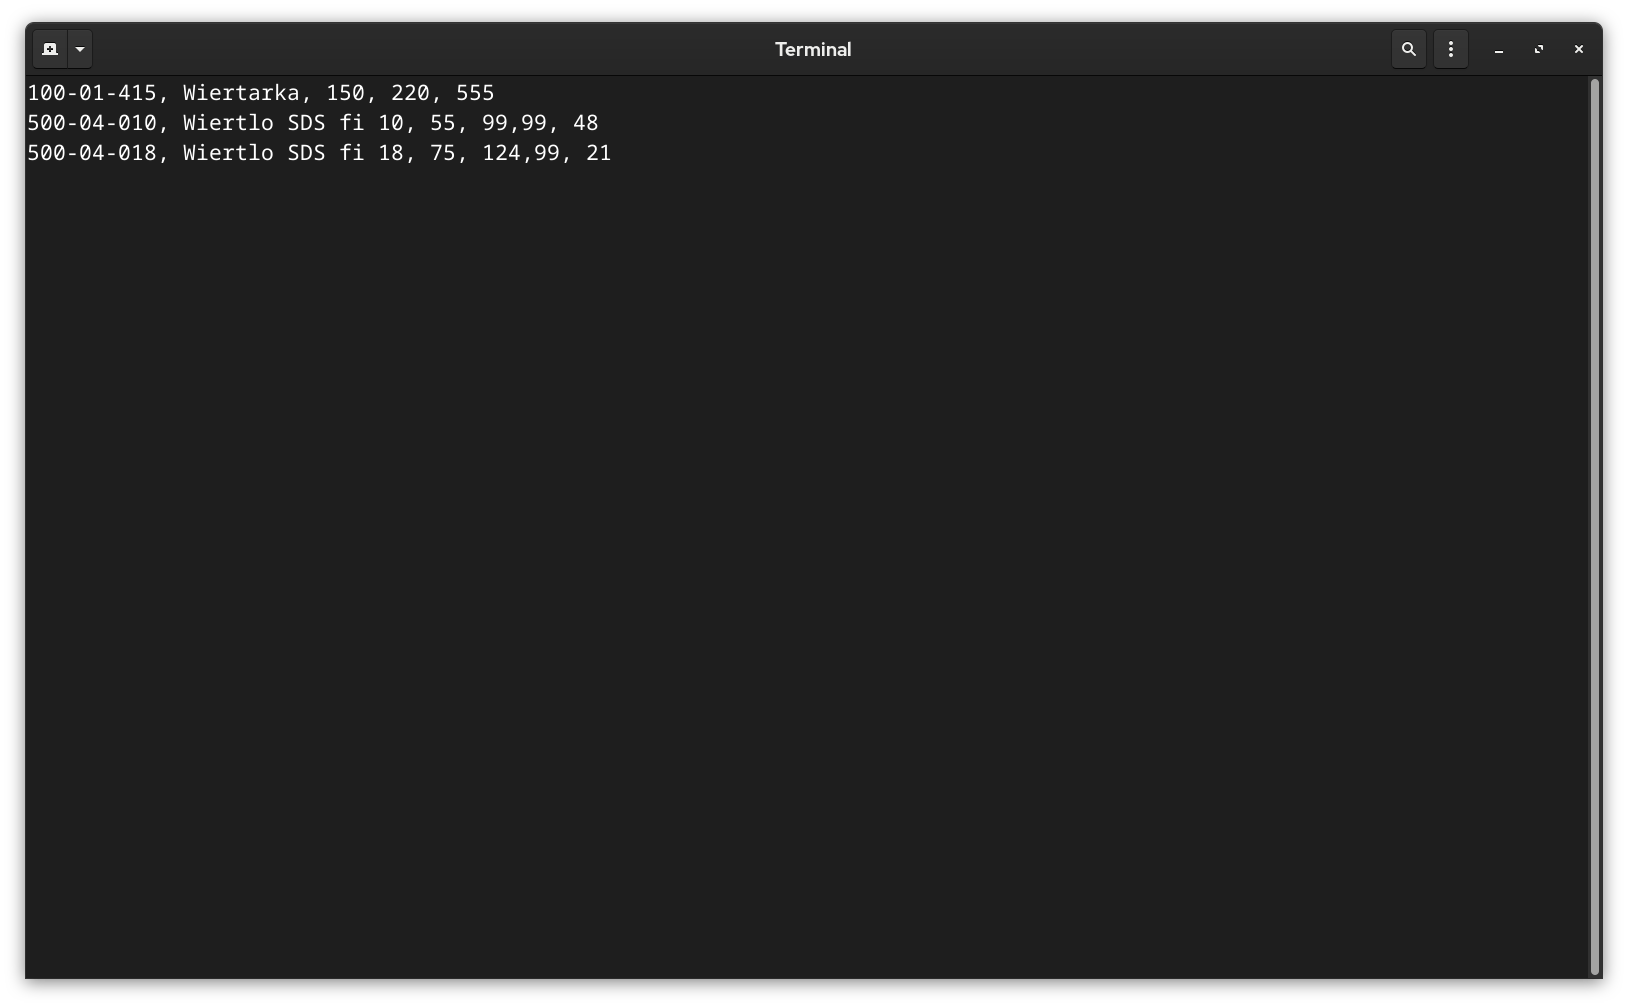
\includegraphics[scale=.30]{figures/ekran_wyszukiwania_2.png}

\caption{Ekran wyszukiwania c.d.}
\end{figure}

\clearpage
\section{Źródła i biblioteki}
\begin{itemize}
    \item \url{https://learn.microsoft.com/en-us/dotnet/standard/data/sqlite/?tabs=netcore-cli}
    \item \url{https://github.com/MV10/dotnet-curses}
    \item \url{https://joshclose.github.io/CsvHelper/}
\end{itemize}

\end{document}
